\chapter{Diagnosis of training and configuration choices}
% Por qué nuestra implementación del esquema original olvida lo aprendido cuando termina la exploración con gamma = 0.99, y cómo el diagnóstico llevó a la configuración de los barridos.
\label{apx:diagnosis}

\looseness=-1 The first runs of our implementation of the original scheme, with $\gamma = 0.99$, showed a problem that the
paper does not report: the reward rises during the first half of training and then drops when exploration
reaches its floor, at episode 1200. In Fig.~10 of \citet{li+22fedmarl}, by contrast, the reward keeps rising up
to episode 4000. With $K = 10$ and seed 0, \ac{FedAvg} reaches 4526 in its best block of 200 episodes and ends
at 3226, 29\% lower (Figure~\ref{fig:res-diagnosis}, gray line). Greedy, in the same scenarios, obtains
5369: the learning scheme ends far below the simplest rule. A diagnosis looked for the cause with 24
variants, organized in six sets, each one asking a single question (Table~\ref{tab:res-diagnosis}). All of
them use \ac{FedAvg}, $K = 10$, and seed 0.

\begin{figure*}[tbp]
  \centering
  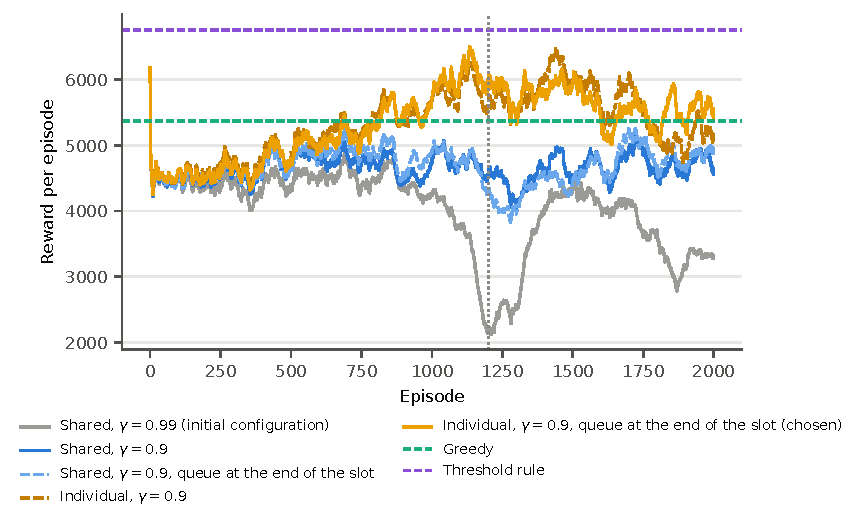
\includegraphics{figures/res_diagnosis.pdf}
  \caption[Diagnosis: learning curves of five variants]{Learning curves of five variants of the diagnosis
    (\acs{FedAvg}, $K = 10$, seed 0), smoothed with a moving average of 50 episodes. The horizontal lines
    are Greedy and the threshold rule in the same scenarios. The dotted vertical line marks episode 1200,
    where exploration reaches its floor.}
  \label{fig:res-diagnosis}
\end{figure*}

\begin{table*}[tbp]
  \centering
  \linespread{1}\footnotesize
  \caption[Results of the diagnosis]{Diagnosis of training (\acs{FedAvg}, $K = 10$, seed 0). ``Peak'' is
    the best mean over a block of 200 episodes, ``Final'' the mean over the last 200, and ``Change'' the
    relative difference between them. The groups are, in order, the sets on the drop, learning, $\gamma$,
    the queue, the reward, and stability. In bold, the chosen configuration. With the same seed, Greedy
    obtains 5369 and the threshold rule 6754.}
  \label{tab:res-diagnosis}
  \begin{tabularx}{\textwidth}{@{}llXrrr@{}}
    \toprule
    Reward & $\gamma$ & Other changes & Peak & Final & Change \\
    \midrule
    \tablerows{tables/res_diagnosis.tex}
    \bottomrule
  \end{tabularx}
\end{table*}

\paragraph{Drop: too little memory or too large a scale?} \looseness=-1 Two common stabilizers soften the drop without
solving the problem. A replay buffer ten times larger, which holds 500 episodes instead of 50, reduces it to
6\%, and multiplying the reward by 0.01, so that the Q values are smaller, reduces it to 20\%. With both
changes at once, the variant ends at 4411, still far below Greedy.

\paragraph{Learning: is it the differences from the paper?} \looseness=-1 The network of \citet{li+22fedmarl}, with layers
of 500, 250, and 120 neurons, ends at 3788, and their exploration floor of 0.1 ends at 3739. Both end
somewhat better than the initial configuration, but neither avoids the drop (17\% and 19\% below their
peaks). So these two differences from the paper do not explain the problem. Two other differences were not
tested with the values of the paper: the learning rate ($10^{-3}$ here, 0.7 there) and how often the agents
learn (every slot here, every 100 slots there). The diagnosis therefore cannot say whether the published
scheme, with its own settings, has this problem.

\paragraph{The discount factor.} \looseness=-1 The change that almost removes the drop is lowering $\gamma$ from 0.99 to
0.9: the variant ends at 4703, only 3\% below its peak. Nearby values confirm it: 0.85 ends at 4653, 0.8 and
0.7 end lower (4320 and 4263), and 0.95 drops again (3329). A possible explanation lies in the scale of the
Q values. With $\gamma = 0.99$, the return weighs about 100 future slots, the horizon $1/(1-\gamma)$ of
Section~\ref{sec:bg-rl}, so the Q values are about a hundred times the reward of one slot. The difference
between staying silent and transmitting in one slot is a tiny fraction of them, and it gets lost in the
estimation error. With $\gamma = 0.9$, the horizon is about 10 slots, and that difference weighs ten times
more. Since \citet{li+22fedmarl} do not give the value of $\gamma$, choosing 0.9 does not depart from the
paper.

\paragraph{Queue: does it matter when the cost is charged?} \looseness=-1 With the shared reward, measuring the queue at
the end of the slot instead of at its start does not change the result. With $\gamma = 0.99$, the variant
drops just the same (3343), and with $\gamma = 0.9$ it ends at 4852, practically the same as without the
change. Adding to the observation the channel that the pair used in the previous slot does not help
consistently either.

\paragraph{Reward: the largest change.} \looseness=-1 The four variants with the individual reward end above all the
variants with the shared reward, and three of them exceed Greedy in their best stretch (peaks of 5788 to
6051). The best one combines the individual reward, $\gamma = 0.9$, and the queue measured at the end of the
slot. It reaches 6051 and ends at 5586, the first configuration that ends above Greedy. With the individual
reward, measuring the queue at the end of the slot does matter (5586 against 5083). 
% This agrees with the
% argument of Section~\ref{sec:pa-individual-reward}: when an agent is judged by its own queue, charging the
% cost in the same slot as the action that caused it makes the link between the two clearer.

\paragraph{Stability: can forgetting be avoided?} \looseness=-1 The best variant still loses 8\% after its peak. On top of
it, a lower learning rate ($3 \times 10^{-4}$ or $10^{-4}$), an exploration floor of 0.1, and a buffer of
100,000 transitions do not improve the final value: the four end between 5126 and 5391. The learning rate of
$3 \times 10^{-4}$ reaches the highest peak, 6234, but forgets just the same.

\paragraph{The chosen configuration.} \looseness=-1 The sweeps use $\gamma = 0.9$ with both rewards. With the individual
reward, the queue is measured at the end of the slot. With the shared reward, it is measured at the start,
as in \citet{li+22fedmarl}, because measuring it at the end did not change its result. 
% Everything else stays
% as in Section~\ref{sec:exp-parameters}.

\enlargethispage{\baselineskip}% the chapter would otherwise end with a single line on the next page
\paragraph{Two caveats.} \looseness=-1 First, the diagnosis uses a single seed, and the variability between runs is large.
The chosen configuration, run again with the same seed in the sweep, ended at 4631 instead of 5586. The
diagnosis ran on a graphics card and the sweep on processors; floating-point computations differ slightly
between the two, and these differences are enough for two trainings to take different paths. For this
reason, the diagnosis only served to choose the configuration, and the conclusions of Chapter~\ref{chap:results}
rest on the sweeps, with three seeds. Second, in the variants that measure the queue at the end of the slot,
the reward was logged with that same change. The difference is small: the logged reward contains the same
queue terms, shifted by one slot, and it differs from the shared reward as defined by at most 55 per episode
with $K = 10$, about 1\% of the values in the table.
